\documentclass{article}
\usepackage[utf8]{inputenc}
\usepackage{amsmath,graphicx,varioref,verbatim,amsfonts,geometry}
\usepackage[hidelinks]{hyperref}
\usepackage{listings}
\usepackage[T1]{fontenc}
\usepackage{mathtools}
\usepackage{textcomp}
\usepackage[english, norsk]{babel}
\usepackage{wrapfig}
\usepackage{fancyhdr}
\usepackage{amssymb}
\usepackage{enumitem}
\usepackage{xcolor}
\usepackage{lastpage}
\usepackage{graphicx}
\usepackage{matlab-prettifier}
\usepackage{filecontents}
\usepackage{underscore}
\usepackage{makecell}
\usepackage{caption}
\usepackage{subcaption}
\usepackage{siunitx}
\usepackage{mathrsfs}

\pagestyle{fancy}


%% Double underline 
\def\dubline#1{\underline{\underline{#1}}}

%% Matrix
\newcommand\SmallMatrix[1]{{%
		\arraycolsep=0.3\arraycolsep\ensuremath{\begin{pmatrix}#1\end{pmatrix}}}}
	
%% Codeinsert
\definecolor{listinggray}{gray}{0.9}
\definecolor{lbcolor}{rgb}{0.9,0.9,0.9}
\lstset{
	backgroundcolor=\color{lbcolor},
	tabsize=4,
	rulecolor=,
	language=python,
	basicstyle=\scriptsize,
	upquote=true,
	aboveskip={1.5\baselineskip},
	columns=fixed,
	numbers=left,
	showstringspaces=false,      
	extendedchars=true,
	breaklines=true,
	prebreak = \raisebox{0ex}[0ex][0ex]{\ensuremath{\hookleftarrow}},
	frame=single,
	showtabs=false,
	showspaces=false,
	showstringspaces=false,
	identifierstyle=\ttfamily,
	keywordstyle=\color[rgb]{0,0,1},
	commentstyle=\color[rgb]{0.133,0.545,0.133},
	stringstyle=\color[rgb]{0.627,0.126,0.941}
}
\newcounter{subproject}
\renewcommand{\thesubproject}{\alph{subproject}}
\newenvironment{subproj}{
	\begin{description}
		\item[\refstepcounter{subproject}(\thesubproject)]
	}{\end{description}}

\begin{document}
\title{IN3190 - Exam Preparation Questions H23\\
{\Large University of Oslo}}
\author{Daniel Tran \& Erik Røset}
\date{November 2023}
\fancyhead[L]{Should know to exam H23 - IN3190}
\fancyhead[C]{UiO}
\fancyhead[R]{Daniel Tran \& Erik Røset}
\cfoot{\thepage\ of \pageref{LastPage}}
\maketitle
\hypersetup{linkcolor=black}
\tableofcontents
\clearpage

\section{Essential Topics}
\subsection{Discrete time}
\subsubsection{Sine, cosine and exponential functions}

    Mathematical formula that establishes the fundamental relationship between the trigonometric functions and the complex exponential function. \newline
    Euler's formula states that for any real number $x$:
    \begin{equation}
        e^{ix} = \cos(x) + i\sin(x)
    \end{equation}
    When $x = \pi$, Euler's formula yields Euler's identity:
    \begin{equation}
        e^{i\pi} + 1 = 0
    \end{equation}
\subsubsection{Elementary discrete signals}
\paragraph{Unit impulse} %Spør gruppelærer om plot fra forelesning
Also known as the dirac delta function. Shifted to the left when its negative and to the right when its positive. Can be used to find H(n) in a system. If the input $x(n) = \delta(n)$, then the output $y(n) = h(n)$.
\begin{equation}
    \delta[n] = \begin{cases}
        1, & n = 0 \\
        0, & n \neq 0
    \end{cases}
    \hspace*{20pt}\text{may also be written as:}
    \hspace*{20pt} \delta[n] = u[n] - u[n-1]
\end{equation}

\begin{figure}[h!]
    \centering
    \includegraphics[width=0.5\textwidth]{figures/Discrete time/unit_impulse.png}
    \caption{Unit impulse}
    \label{fig:unit_impulse}
\end{figure}

\paragraph{Step function}
Also known as unit step, unit step function or heaviside function. The value which is zero for negative arguments and one for positive arguments.
\begin{equation}
    u[n] = \begin{cases}
        1, & n \geq 0 \\
        0, & n < 0
    \end{cases}
    \hspace*{20pt}\text{may also be written as:}
    \hspace*{20pt} u[n] = \sum_{k=0}^{\infty} \delta[n-k]
\end{equation}
\begin{figure}[h!]
    \centering
    \includegraphics[width=0.5\textwidth]{figures/Discrete time/unit_step_function.png}
    \caption{Unit step function}
    \label{fig:unit_step}
\end{figure}

\newpage
\paragraph{Ramp function}
Also known as the unit-ramp or unit ramp function. Graph shaped like a ramp.
\begin{equation}
u_r[n] = \begin{cases}
    n, & n \geq 0 \\
    0, & n < 0
\end{cases}
\end{equation}
\begin{figure}[h!]
    \centering
    \includegraphics[width=0.5\textwidth]{figures/Discrete time/unit_ramp_function.png}
    \caption{Unit ramp function}
    \label{fig:unit_ramp}
\end{figure}

\paragraph{Periodic sequences} 
$x[n]$ is periodic if and only if $x[n] = x[n+N]$
\begin{itemize}
    \item \textbf{Fundamental period}: 
    \newline Smallest positive integer N which fulfills the relation above
    \item \textbf{Sinusoidal sequences}: 
    \newline $x[n] = A\cos(\omega_0n + \phi)$, where 
    \begin{itemize}
        \item $A$ is amplitude,
        \item $\omega_0$ is the angular frequency
        \item and $\phi$ is the phase of $x[n]$.
    \end{itemize} 
    $x[n]$ is periodic if and only if $\omega_0N = 2\pi k$, for N and k as positive integers.
\end{itemize}

\begin{figure}[h!]
    \centering
    \includegraphics[width=0.5\textwidth]{figures/Discrete time/sinusoidal_sequences.png}
    \caption{Sinusoidal sequences}
    \label{fig:Sinusoidal_sequence}
\end{figure}

\subsubsection{LTI systems, including characteristics via the transformation between input and output}
\paragraph{Linearity:} The relationship between the input $x(t)$ and the output $y(t)$, both being regarded as functions. If $a$ is a constant then the system output to $ax(t)$ is $ay(t)$. Linear system if and only if it $H\{\cdot\}$ is both additive and homogeneous, in other words: If it fulfills the superposition principle. That is:
\begin{equation}
    H\{ax_1(t)+bx_x(t)\} = aH\{x_1(t)\} + bH\{x_2(t)\}
\end{equation}

\paragraph{Time-invariance:} 
A linear system is time-invariant or shift-invariant means that wether we apply an input to the system now or T seconds from now, the output will be identical except for a time delay of S seconds. In other words, if $y(t)$ is the output of a system with a input $x(t)$, then the output of the system with input $x(t-T)$ is $y(t-T)$. The system is invariant becasue the output does not depend on the particular time at which the input is applied.
\\
\\
The fundamental result in LTI system theory is that any LTI system can be characterized entirely by a single function called the system's impulse response $h(t)$. The output of the system $y(t)$ is simply the convolution of the input to the system $x(t)$ with the systems's impulse response $h(t)$.
\\
\\
LTI system can also be characterized in the frequency domain by the system's transfer function $H(s)$, which is the Laplace transform of the system's impulse response $h(t)$. Or Z-transform in the case of discrete time systems.
\begin{figure}[h!]
    \centering
    \includegraphics[width=0.5\textwidth]{figures/Discrete time/LTI_time_freq_domain.png}
    \caption{Relationship between the time domain and the frequency domain}
    \label{fig:lti_relationship}
\end{figure}

\subsubsection{Difference equations for system description / LTI systems written on general summation notation with coefficients and time offsets} %Ask why M
General description of relationship between input x[n] and output y[n] of a LTI system in the time domain (n domain): (M amount of zeroes) (N amount of poles)
\begin{equation}
    y[n] = -\sum_{k=1}^{N}a_ky[n-k] + \sum_{k=0}^{M}b_xx[n-k]
\end{equation}
\begin{itemize}
    \item FIR (finite impulse response): all $a_k = 0$
    \item IIR (infinite impulse response): at least one $a_k \neq 0$
\end{itemize}
The value N represent the order of the difference equation and corresponds to the memory of the system being represented. Because this equations relies on past values of the output, in order to compute a numerical solution, certain past outputs, referred to as the initial conditions, must be known.
\\
\textbf{$a_k$} and \textbf{$b_k$} are the coefficients of the difference equation. 
Time offset is represented by the index k.

\subsubsection{Casuality}
In control theory, a causal system is a system where the output depends on past and current inputs, but not future inputs. The idea that the output of function at any time depends only on past and present values of input is defined by the property commonly referred to as casusality. 

\subsubsection{Stability and the related convergence for the DTFT}
A linear system is called BIBO (Bounded-input bounded output) stable if its output will stay bounded for any bounded input. 

\paragraph{Discrete-time signals:} For a rational and discrete time system, the conditon for BIBO stability  is that the ROC (region of convergence) of the z-transform includes the unit circle. When the system is causal, the ROC is the open region outside a circle whose radius is the magnitude of the pole with largest magnitude. Therefore, all poles of the system must be inside the unit circle in the z-plane for BIBO stability. For stable systems, the unit circle is part of ROC. 
\\
\\
Causal stable filters have all poles inside $|z| = 1$.

\subsubsection{FIR / IIR}
\paragraph{FIR:} Finite impulse response. The output from a FIR filter is calculated by the basis of the input samples and the proceding input. A FIR filter is always stable because the values from the output does not effect calculations. 
(Can be thought of as an op-amp without feedback loop)


\paragraph{IIR:} Infinite impulse response. The output from a IIR filter is calculated by the basis of the input samples, the proceding input and the previous output. A IIR filter can be unstable because the values from the output effects the calculations. 
(Can be thought of as an op-amp with feedback loop)

\subsubsection{Convolution}
The resulting signal y(n) represents the amount of overlap between x and h at each point in time, and can be used for a variety of purposes, such as filtering, smoothing, deconvolution, and image processing. For example, if we convolve a signal with a smoothing kernel, we can reduce noise and make the signal smoother.
\\
The summation:
\begin{equation}
    y(n) = \sum_{k=-\infty}^{\infty}x(k)h(n-k) = \sum_{k=-\infty}^{\infty}x(n-k)h(k)
\end{equation}
is the convolution of $x(n)$ and $h(n)$

\paragraph{Properties of convolution:}
\begin{itemize}
    \item \textbf{Commutative:} $x(n) \ast h(n) = h(n) \ast x(n)$
    \item \textbf{Associative:} $x(n) \ast \{h_1(n) \ast h_2(n)\} = \{x(n) \ast h_1(n)\} \ast h_2(n)$
    \item \textbf{Distributive:} $x(n) \ast \{h_1(n) + h_2(n)\} = x(n) \ast h_1(n) + x(n) \ast h_2(n)$
    \\
    where $\ast$ is the convolution operator
    \item Can also use the matrix method to calculate convolution
\end{itemize}
\begin{figure}[h!]
    \centering
    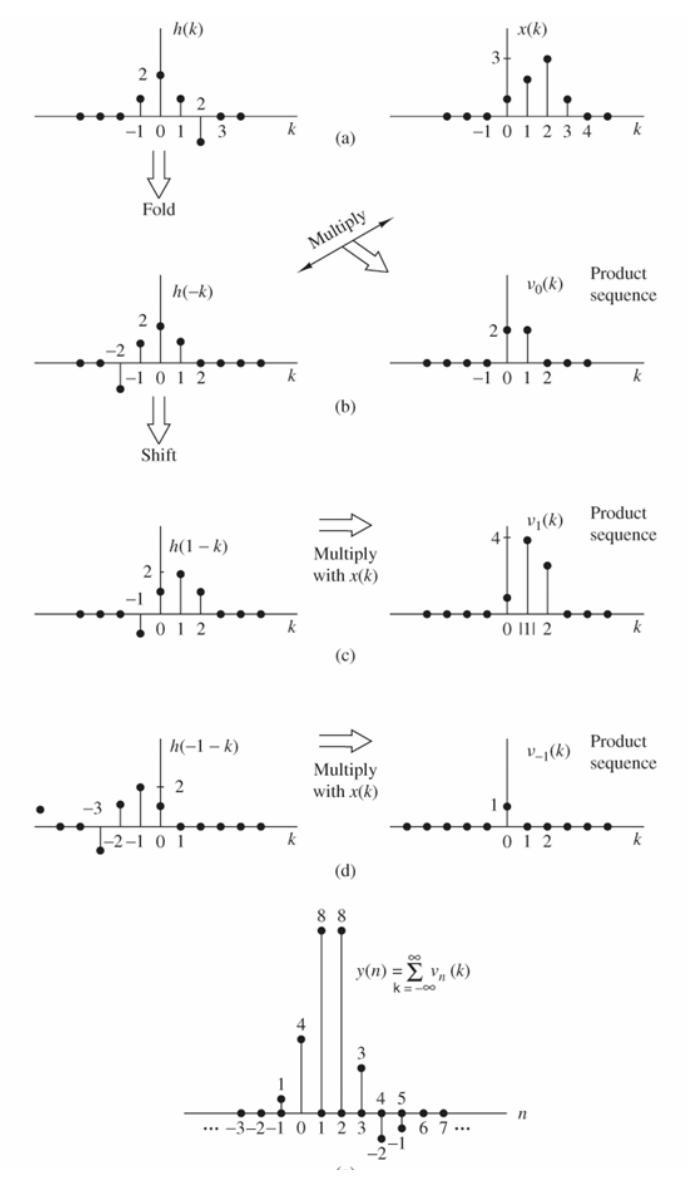
\includegraphics[width=0.5\textwidth]{figures/Discrete time/graphic_conovlution.png}
    \caption{Convolution}
    \label{fig:convolution}
\end{figure}

\subsubsection{Sampling frequency and sampling interval. Digital frequency / physical frequency, as well as
corresponding digital angular frequency / physical angular frequency and how to map between these
given a sampling interval T = 1/FT}

\paragraph{Sampling frequency:}
The sampling frequency or sampling rate, $f_s$ is the average number of samples obtained in one second (samples per second), thus $f_s = 1/T_s$ given in Hz or kHz. To avoid aliasing, the sampling frequency must be greater than twice the maximum frequency of the signal being sampled, according to the Nyquist–Shannon sampling theorem.

\paragraph{Sampling interval:}
The sampling interval or sampling period, $T_s$ is the time between samples, and is equal to the inverse of the sampling frequency $T_s = 1/f_s$. The sampling interval should be chosen small enough to avoid aliasing, but large enough to get a reasonable signal-to-noise ratio.

\paragraph{Physical Frequency} $F[Hz]$

\paragraph{Physical angular frequency} $\Omega = 2\pi F [rad]$

\paragraph{Digital(Normalized) angular frequency} $\omega = \frac{\Omega}{F_T} =  \frac{2\pi F}{F_T} [rad/sample]$

\paragraph{Mapping} $\frac{F}{F_T}$ or $\frac{\Omega}{F_T}$, this is the digital frequency


\subsection{Z-transform}

\subsubsection{Definition and how to derive the various z-transform properties}
\paragraph{Definition:}
The Z-transform(z-domain) is a discrete-time equivalent of the Laplace transform(s-domain). It is a linear transformation of a discrete-time signal which maps a complex-valued discrete-time signal $x[n]$ to a complex-valued function of a complex variable $X(z)$.
\begin{equation}
    X(z) = \mathcal{Z}[x[n]] = \sum_{n=-\infty}^{\infty} x[n]z^{-n}
\end{equation}

\subsubsection*{Propterties}

\paragraph{Linearity:}
If $x[n] \xLeftrightarrow{Z.T} X(z)$ and $y[n] \xLeftrightarrow{Z.T} Y(z)$, then linearity property states that:
\begin{equation}
    ax[n] + by[n] \xLeftrightarrow{Z.T}  aX(z) + bY(z)
\end{equation}

\paragraph{Time shifting:}
If $x[n] \xLeftrightarrow{Z.T} X(z)$, then time shifting property states that:
\begin{equation}
    x[n-m] \xLeftrightarrow{Z.T} z^{-m}X(z)
\end{equation}

\paragraph{Time reversal:}
If $x[n] \xLeftrightarrow{Z.T} X(z)$, then time reversal property states that:
\begin{equation}
    x[-n] \xLeftrightarrow{Z.T} X(z^{-1})
\end{equation}

\paragraph{Scaling in the z-domain:} 
If $x[n] \xLeftrightarrow{Z.T} X(z)$, then scaling property states that:
\begin{equation}
    a^nx[n] \xLeftrightarrow{Z.T} X(a^{-1}z)
\end{equation}
for any constant $a$, real or complex.

\paragraph{Differentiation in the z-domain:}
If $x[n] \xLeftrightarrow{Z.T} X(z)$, then differentiation property states that:
\begin{equation}
    x[n] \xLeftrightarrow{Z.T} \left [-z\frac{dX(z)}{dz} \right ]^k
\end{equation}

\paragraph{Convolution of two sequences:} 
If $x[n] \xLeftrightarrow{Z.T} X(z)$ and $y[n] \xLeftrightarrow{Z.T} Y(z)$, then convolution property states that:
\begin{equation}
    x[n] \ast y[n] \xLeftrightarrow{Z.T} X(z)Y(z)
\end{equation}

\subsubsection{Region of convergence (ROC)}
The region of convergence, known is ROC, is important to understand because it defines the region where the z-transform exist.
\begin{equation}
    ROC = \left \{z:\left|\sum_{n=-\infty}^{\infty}x[n]z^{-n} \right| < \infty \right \}
\end{equation}
\begin{itemize}
    \item ROC cannot contain any poles
    \item ROC tells us if the system is causal and/or stable
    \item From ROC, a system is causal if it goes to $\infty$
    \item If the ROC contains the unit circle, then the system is stable.
\end{itemize}

\subsubsection{Poles/zeroes as well as the connection to stability/causality/symmetry/real signals/frequency response/filter type/linear phase etc}
The poles and zeros from a system is obtained by finding the roots of the transfer functions denominator and numerator respectivily.  $H(s) = \frac{Numerator}{Denominator} = \frac{zeros}{poles}$. The position of the poles can tell us if the system is stable and/or causal. If we also know the position to the zeroes, we can get the mangnitude and phase response of the system. And fram that we can get the filter type and linear phase.
\\
A FIR filter has a perfect linear phase. This means that the phase response of the filter is a linear function of frequency.

\subsubsection{Calculation of H(z) from difference equation and from filter structures}
\paragraph{From difference equation:} 
\begin{equation}
    H(z) = \frac{Y(z)}{X(z)} = \frac{\sum_{k=0}^{M}b_kz^{-k}}{\sum_{k=0}^{N}a_kz^{-k} }= \frac{\mathcal{Z}\{y(n)\}}{\mathcal{Z}\{x(n)\}}
\end{equation}
where $x(n)$ is the input and $y(n)$ is the output. And $X(z)$ and $Y(z)$ is the z-transform of $x(n)$ and $y(n)$ respectivily. 

\subsubsection{Connection between z-transform and DTFT and the associated relationship between $H(z)$ and $H(\omega)$}

\paragraph{Z-transform} $\mathcal{Z}[x(n)] = X(z) = \sum_{n=-\infty}^{\infty}x(n)z^{-n}$ where z is a complex variable given by $z = re^{j\omega}$
\paragraph{DTFT} $F[x(n)] = X(\omega) = \sum_{n=-\infty}^{\infty}x(n)e^{-j\omega n}$

\paragraph{Relationship between $H(z)$ and $H(\omega)$:} $\mathcal{Z}[x(n)] = F[x(n)r^{-n}]$
\begin{itemize}
    \item Z-transform is a generalization of the DTFT
    \item Z-transform is valid for all types of signal (periodic, increasing, decreasing, etc.)
    \item DTFT is valid only for signals that are absolutely summable or has finite energy
\end{itemize}

\clearpage
\subsubsection{The magnitude of $H(\omega)$ from a pole-zero diagram}
Poles in the PZ-plot will make the magnitude rise, while the zero will make the magnitude fall. 
\begin{figure}[h!]
    \centering
    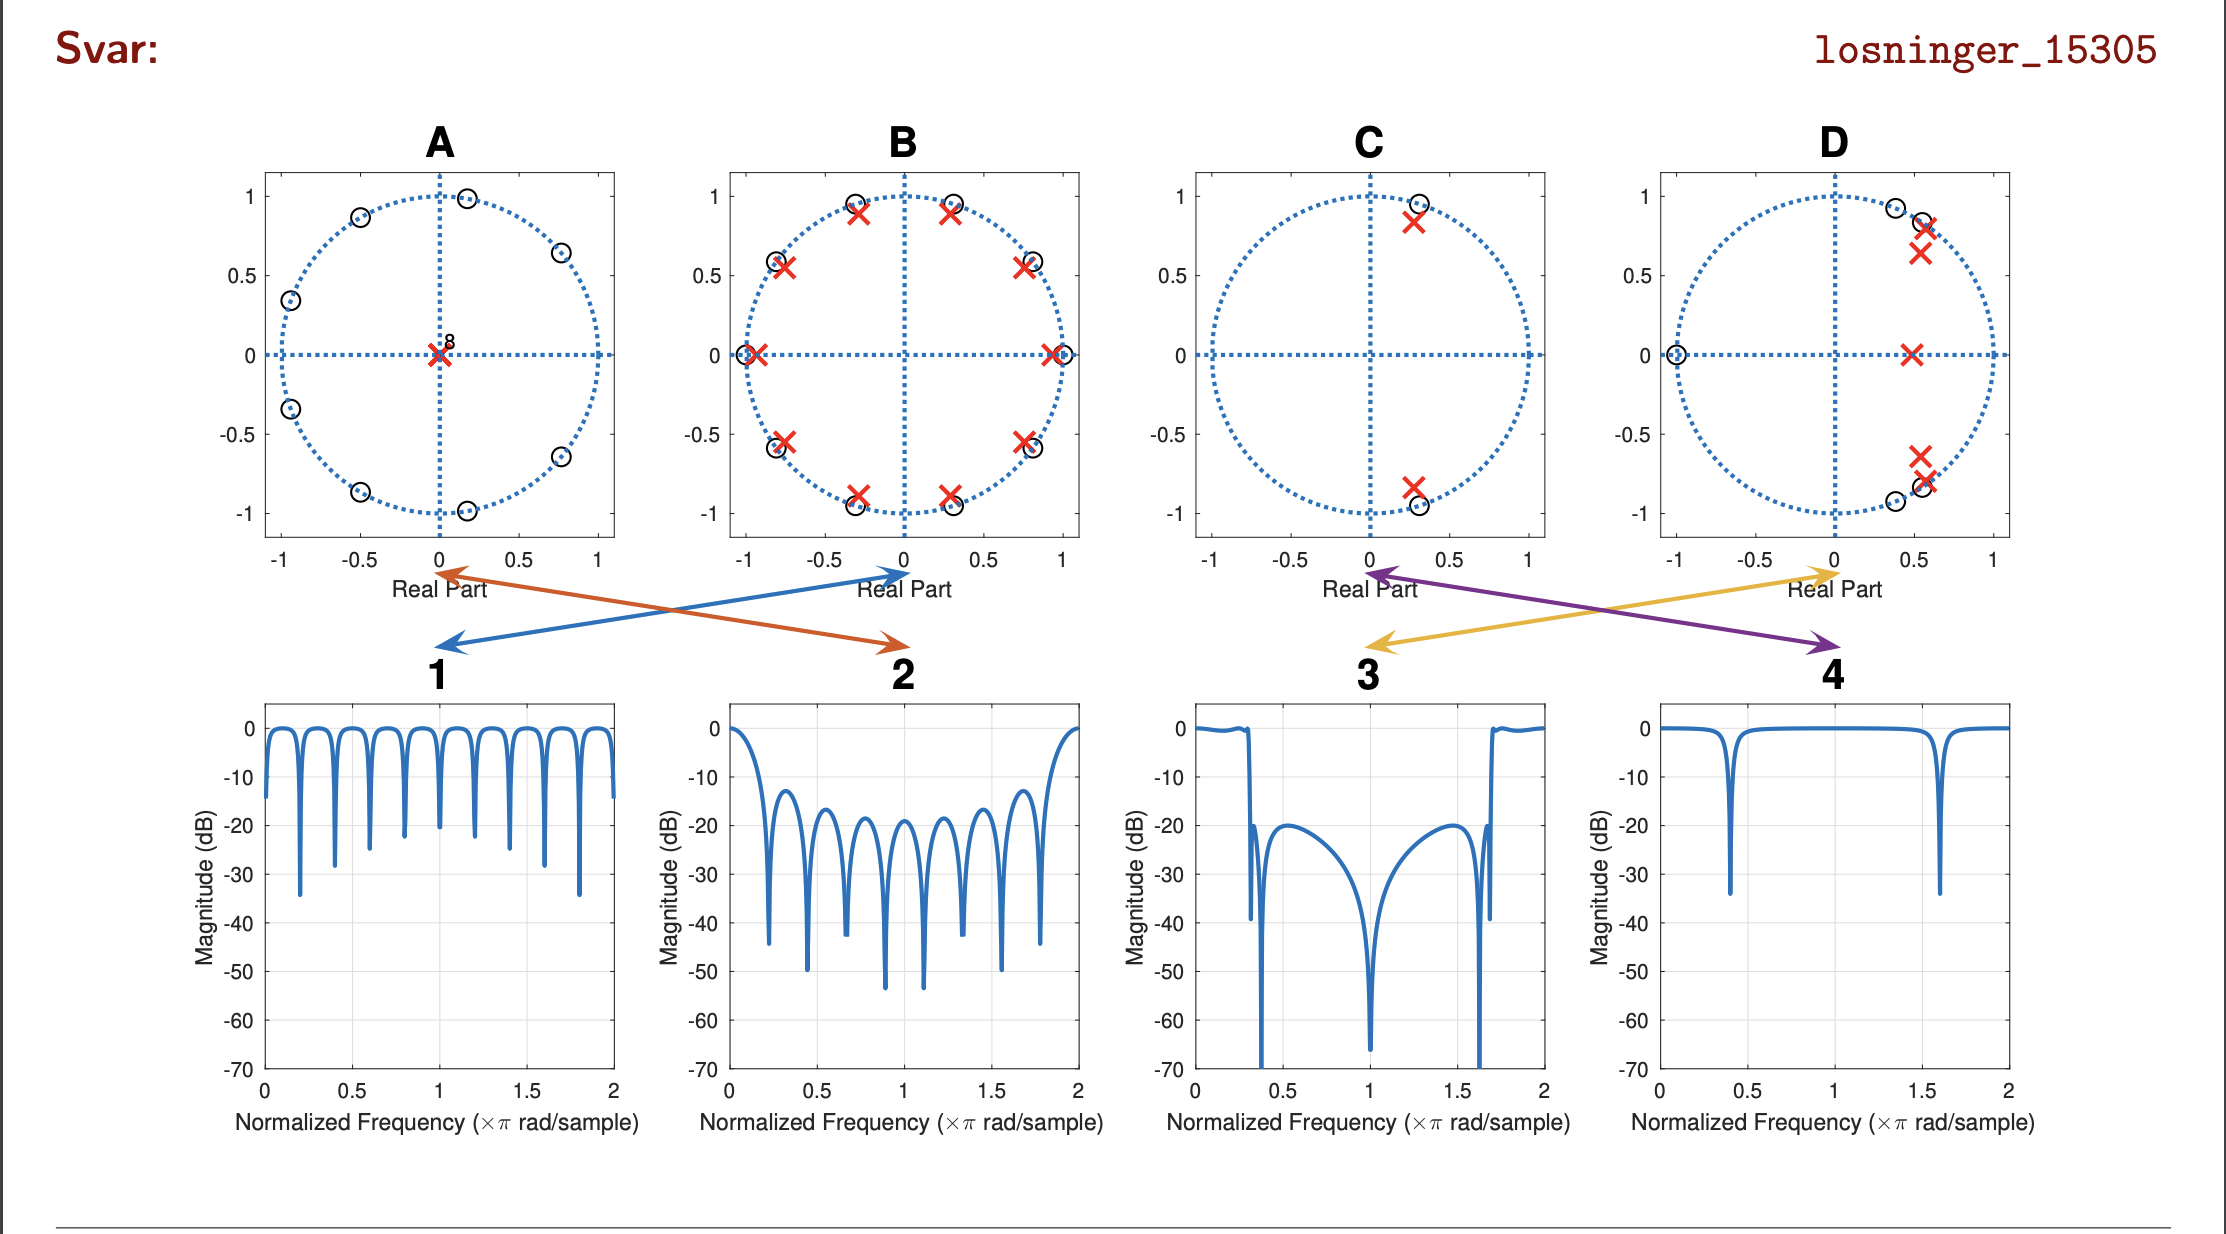
\includegraphics[width=0.8\textwidth]{figures/Z-transform/PZ_magnitude_exam1.png}
    \caption{Pole-zero diagram and corresponding magnitude response exam 1}
    \label{fig:pole_zero_diagram_exam1}
\end{figure}
\begin{figure}[h!]
    \centering
    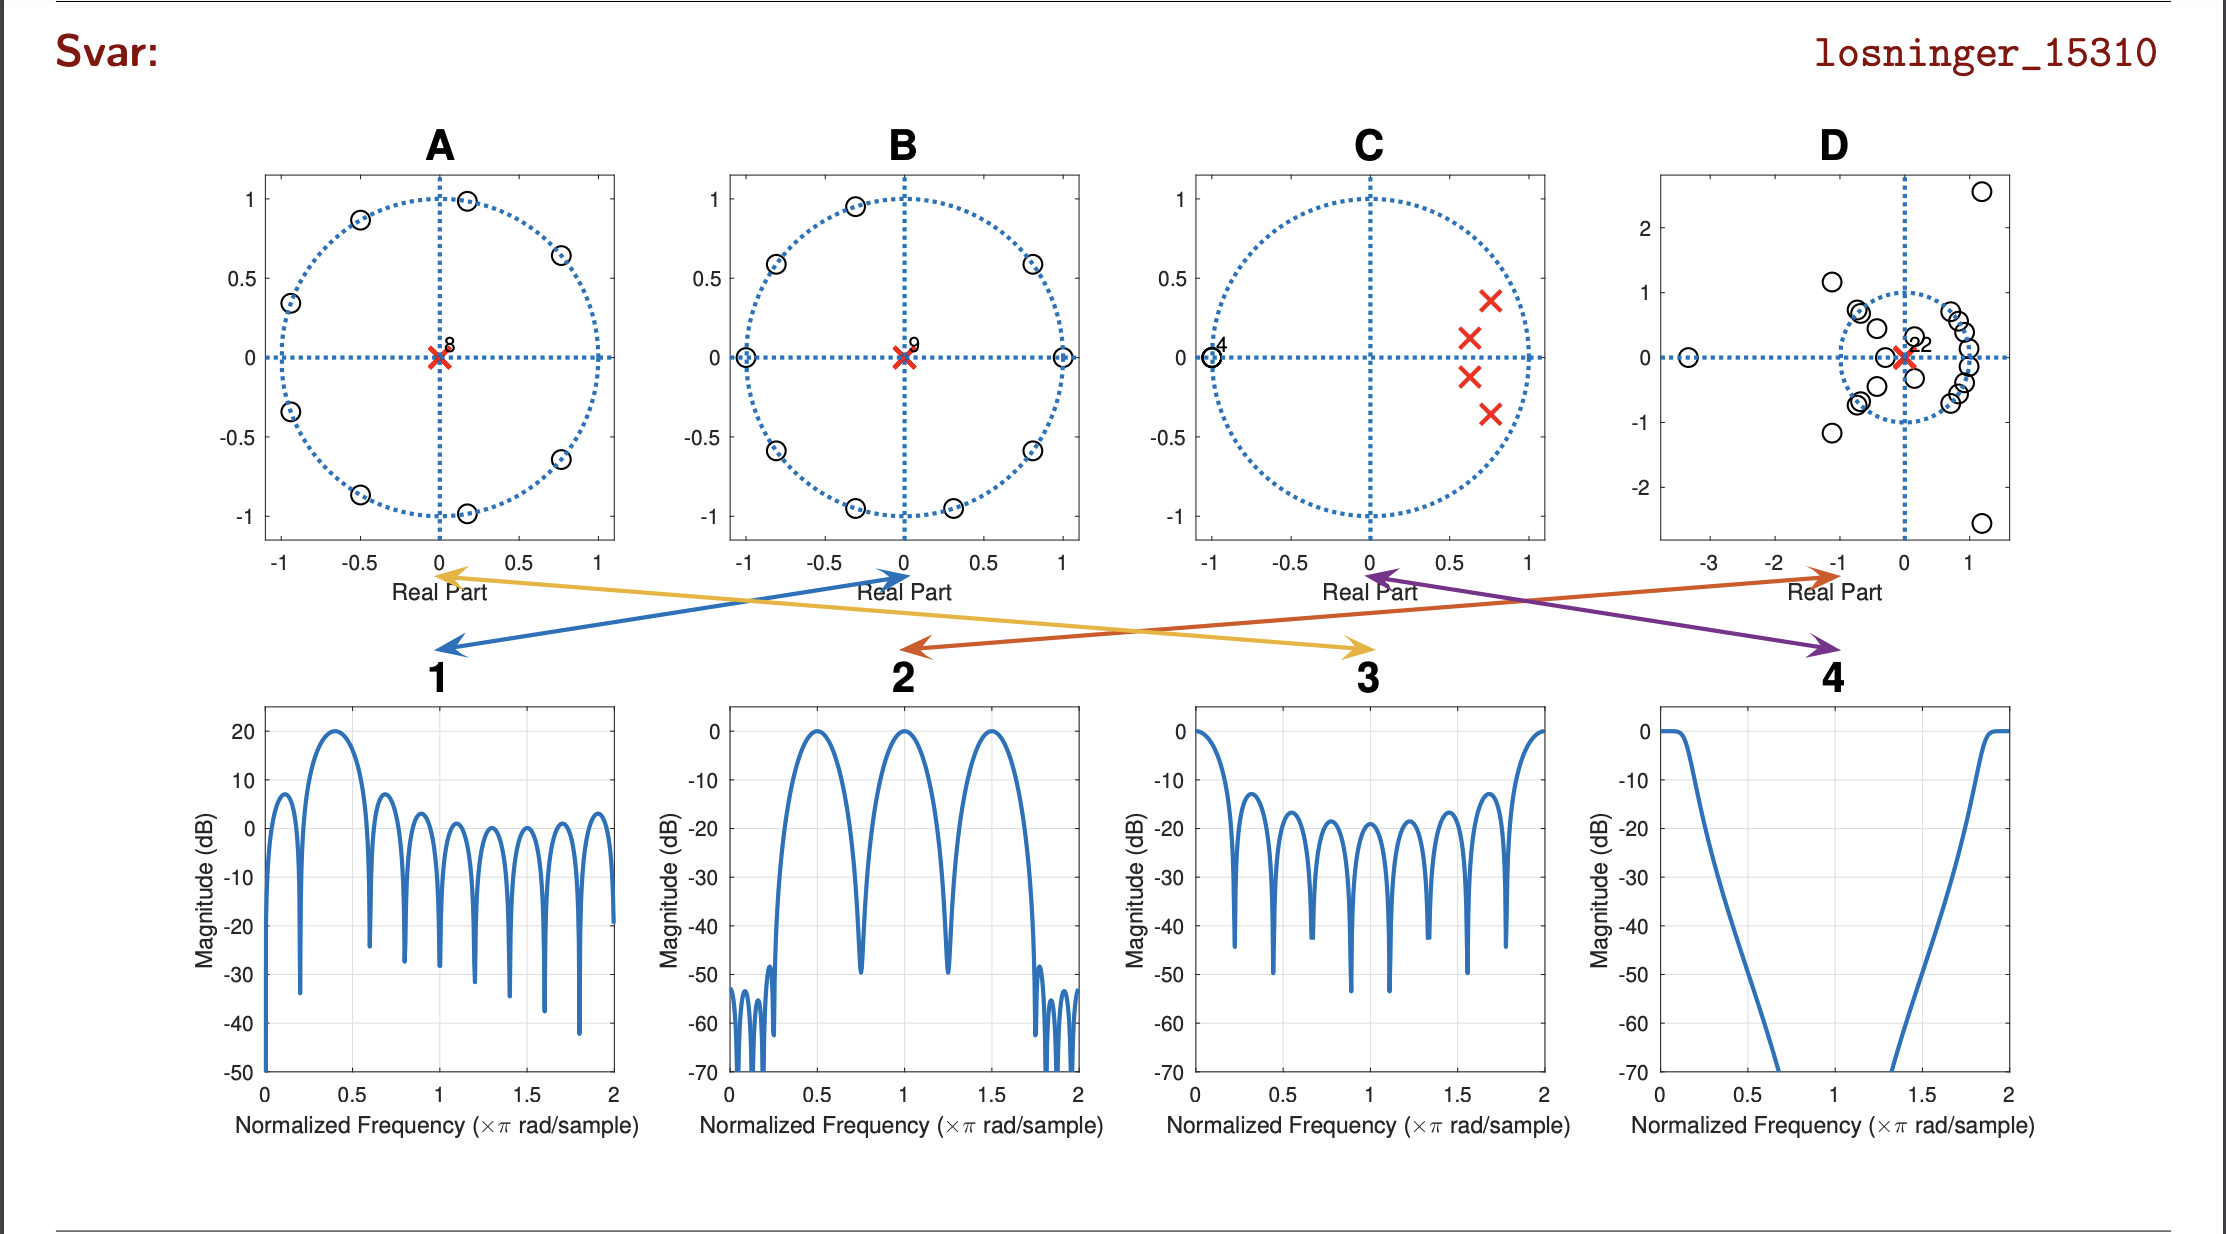
\includegraphics[width=0.8\textwidth]{figures/Z-transform/PZ_magnitude_exam2.png}
    \caption{Pole-zero diagram and corresponding magnitude response exam 2}
    \label{fig:pole_zero_diagram_exam2}
\end{figure}

\clearpage
\subsubsection{Inverse Z-transfrom and approaches that can be used to calculate it}
There are four approcahes to calculate the inverse Z-transform:
\begin{enumerate}
    \item \textbf{Using table:} 
    \begin{itemize}
        \item This is a simple and preferred solution
        \item Should always be considered
        \item Remember the ROC and it's implications
    \end{itemize}
    \item \textbf{Cauchy's countour integral (difficult):}
    \begin{itemize}
        \item It is possible to calculate the inverse Z-transfrom by
        \begin{equation}
            x(n) = \mathcal{Z}^{-1}\{X(z)\} = \frac{1}{2\pi j} \oint_C X(z)z^{n-1}dz
        \end{equation}
        i. e. integrate a long a closed curve in the ROX, where the curve envelops the origin.
        \item This is a difficult method, and should only be used if the other methods are not possible.
    \end{itemize}
    \item \textbf{Power series expansion}
    \item \textbf{Partial fraction expansion}
\end{enumerate}

\clearpage

\subsection{Frequency analysis and DFT}

\subsubsection{DTFT and its central properties}

\paragraph{Discrete time Fourier transform (DTFT):} The DTFT of a discrete-time signal $x[n]$ is defined as:
\begin{align}
    \text{Synthesis equation:} \quad & x[n] = \frac{1}{2\pi} \int_{-\pi}^{\pi} X(e^{j\omega})e^{j\omega n} d\omega \\
    \text{Analysis equation:} \quad & X(e^{j\omega}) = \sum_{n=-\infty}^{\infty} x[n]e^{-j\omega n}
\end{align}
\begin{itemize}
    \item $X(e^{j\omega})$ unique ocer the frequency interval ($-\pi,\pi$), or equivalently ($0,2\pi$)
    \item $X(e^{j\omega})$ is periodic with period $2\pi$
\end{itemize}

\begin{figure}[h!]
    \centering
    \begin{tabular}{|c c c|}
        \hline
        Property & Time domain & Frequency domain \\
        \hline
        Notation & $x[n]$ & $X(\omega)$ \\
        & $x_1(n)$ & $X_1(\omega)$ \\
        & $x_2(n)$ & $X_2(\omega)$ \\
        \\
        Linearity & $ax_1(n) + bx_2(n)$ & $aX_1(\omega) + bX_2(\omega)$ \\
        Time shifting & $x(n-k)$ & $e^{-j\omega k}X(\omega)$ \\
        Time reversal & $x(-n)$ & $X(-\omega)$ \\
        Convolution & $x_1(n) \ast x_2(n)$ & $X_1(\omega)X_2(\omega)$ \\
        Parseval's theorem & $\sum_{n=-\infty}^{\infty}x(n)y^*(n)$ & $\frac{1}{2\pi}\int_{-\pi}^{\pi}X(\omega)Y^*(\omega)d\omega$ \\
        \hline
    \end{tabular}
    \caption{Properties of DTFT}
    \label{table:DTFT_properties}
\end{figure}

\subsubsection{DFT}
\paragraph{Discrete Fourier transform (DFT):} 

The DFT converts a finite sequence of equally-spaced samples of a function into a same-length sequence of equally-spaced samples of the discrete-time Fourier transform (DTFT). The DTFT is the sampled Fourier transform of the function $x(n)$, and is itself a periodic summation of the Fourier transform of the function $x(n)$.

The DFT of a discrete-time signal $x[n]$ is defined as:

\begin{align}
    \text{DFT of } N\text{-length signal:} \quad & X(k) = \sum_{n=0}^{N-1} x[n]e^{-j\frac{2\pi}{N}kn} \\
    \text{Inverse DFT of } N\text{-length signal:}  \quad & x(n) = \frac{1}{N}\sum_{k=0}^{N-1} X(k)e^{j\frac{2\pi}{N}kn}
\end{align}

\subsubsection{Relationship between DFT and DTFT}

\begin{align}
    \begin{matrix}
        \textcolor{red}{\text{DFT:}} & X(k) = \textcolor{red}{\sum_{n=0}^{N-1}} x(n)e^{-j\textcolor{red}{\frac{2\pi k}{N}}n} & x(n) = \frac{1}{N}\textcolor{red}{\sum_{k=0}^{N-1}}X(k)e^{j\textcolor{red}{\frac{2\pi K}{N}}n} \\ \\
        \textcolor{red}{\text{DTFT:}} & \tilde{X}^(e^{j\omega}) = \textcolor{red}{\sum_{n=-\infty}^{\infty}} x(n)e^{-j\textcolor{red}{\omega} n} & x(n) = \frac{1}{2\pi}\textcolor{red}{\int_{0}^{2\pi}}\tilde{X}(e^{j\omega})e^{jpl \textcolor{red}{\omega} n} d\omega
    \end{matrix}
\end{align}

Using $\omega = \frac{2\pi k}{N}$ and $x(n)$ is a finite discrete sequence of length $N$, or $x(n)$ is one period of a periodic discrete sequence of length $N$, the the DFT and DTFT are \textbf{exactly equal}. Else the DFT is just a approximation of the DTFT.
\subsubsection{The four Fourier transforms}

\begin{figure}[h!]
    \centering
    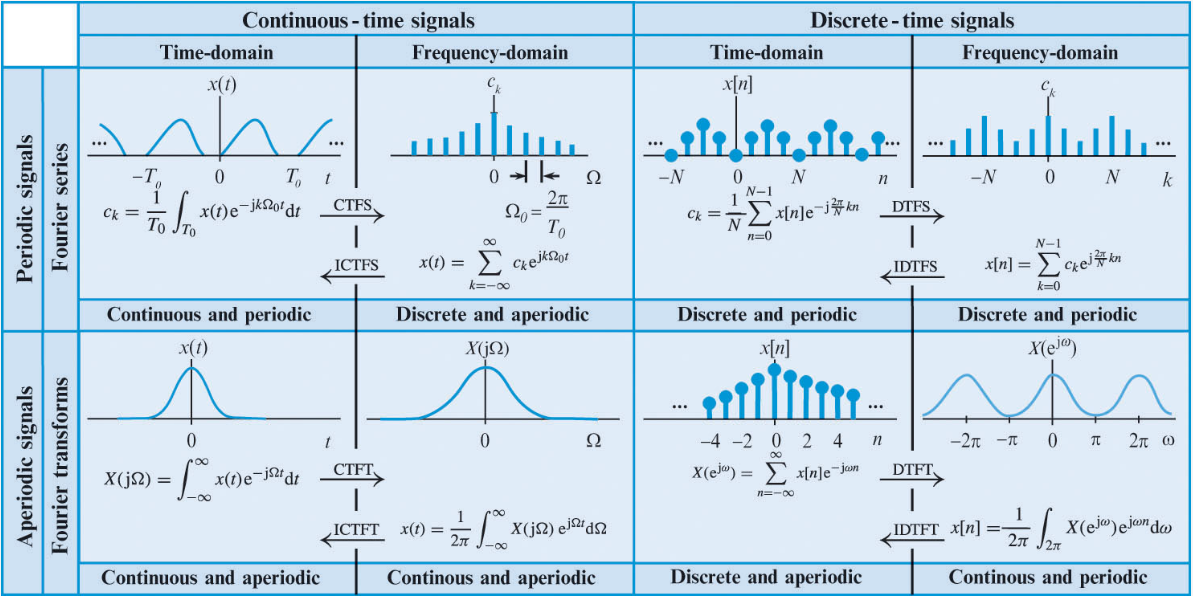
\includegraphics[width=0.8\textwidth]{figures/DFT/fourier_reps.png}
    \caption{The four Fourier transforms}
    \label{fig:furry_transforms}
\end{figure}

\begin{itemize}
    \item \textbf{CTFS} Continiuous and periodic in the time domain, discrete inn the Fourier domain.
    \item \textbf{CTFT} Fourier transfrom for continuous time non-periodic signals.
    \item \textbf{DTFS} Discrete and periodic in the time domain, discrete and periodic in the Fourier domain.
    \item \textbf{DTFT} Fourier transform for discrete time non-periodic signals.
\end{itemize}

\clearpage

\subsubsection{Ideal filters}

\begin{figure}[h!]
    \centering
    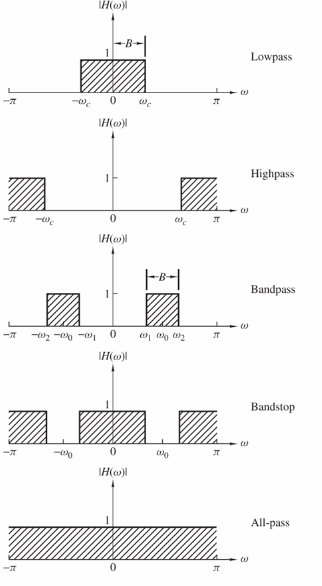
\includegraphics[width=0.3\textwidth]{figures/DFT/ideal_filters.png}
    \caption{Ideal filters}
    \label{fig:ideal_filters}
\end{figure}


\subsubsection{Min/max/mixed phase and inverse system}
\paragraph{Min phase:}
\begin{itemize}
    \item A minimum phase system has a minimized phase responsne for a given magnitude response.
    \item The system has the minimum possible group delay for a given magnitude response. This means the system responds to changes in frequecy as quickly as possible.
    \item Practically, min. phase systems are often associated with systems that are causal and stable.
    \item \textbf{FIR systems} has all zeros within the unit circle, \textbf{IIR systems} has all poles and zeros within the unit circle.
\end{itemize}

\paragraph{Max phase:}
\begin{itemize}
    \item A maximum phase system has a maximized phase response for a given magnitude response.
    \item The system has the maximum possible group delay for a given magnitude response. This means the system responds to changes in frequency as slowly as possible.
    \item \textbf{FIR systems} All zeros outside the unit circle, \textbf{IIR systems} All zeros outside the unit circle and all poles inside the unit circle. (I.e. stable and causal.)
\end{itemize}

\paragraph{Mixed phase:}
\begin{itemize}
    \item Has min. and max. components.
    \item This mean the system can exhibit characteristics from both types, depending on frequency.
\end{itemize}

\paragraph{Inverse system:}
Inverse system are designed to reverse the effect of a system. This type of systems can be suggest by cascasding a system with its inverse will reverse the output back to the input.
 Some consequenses of inverse systems are:
\begin{itemize}
    \item \textbf{FIR:} $H_1(z) = B(z)$, then $H_2(z)=H_1^{-1}(z) = \frac{1}{B(z)}$ I.e. IIR
    \item \textbf{IIR:} $H_1(z) = \frac{1}{A(z)}$, then $H_2(z)=H_1^{-1}(z) = A(z)$ I.e. FIR 
    \item \textbf{IIR:} $H_1(z) = \frac{B(z)}{A(z)}$, then $H_2(z) = H_1^{-1} = \frac{A(z)}{B(z)}$ I.e. IIR
\end{itemize}

\paragraph{Consequences:}
\begin{itemize}
    \item Poles in $H_1(z)$ become zeros in $H_2(z)$ and vice versa.
    \item The ROC of an inverse system is determined by the requirement that $H_1(z)$ and $H_2(z)$ must have overlapping ROC.
    \item $H_2(z)$ does not need to end up being stable or implementable. (Unstable and non-causal)
    \item $H_2(e^{j\omega})$ is not necessarily existing.
\end{itemize} 

\subsubsection{Circular and linear convolution}
\paragraph{Circular convolution:}
\begin{equation}
    x[n] \circledast h[n] \xleftrightarrow{DFT} X[k]H[k]
\end{equation}
\begin{itemize}
    \item Circular convolution is essentially the same process as linear convolution. However, in circular convolution, the signals are all periodic.
    \item In circular convolution, both the sequences (input and impulse response) must be of equal sizes. They must have the same number of samples. Thus the output of a circular convolution has the same number of samples as the two inputs. If the two signals are not of equal sizes, then the convolution is only possible after modifying the signals with a method known as zero-padding
    \begin{itemize}
        \item \textbf{Zero-padding:} Zero-padding is a technique which can be used to equalize the lengths of two signals in order to perform circular convolution. It is done by adding zeros to the end of the shorter signal until it is the same length as the longer signal.
    \end{itemize}
    \item The output of a circular convolution is always periodic, and its period is specified by the length of the input sequences.
\end{itemize}

\subsubsection{Advantages of FFT. The computational complexity to DFT to definition}

The DFT requires $N^2$ operations to compute $N$. The FFT requires $N \log_2 N$ operations for the same results.
\subsection{Filter design}

\subsubsection{Advantages/Disadvantages of FIR and IIR filters}
\paragraph{Advantages, FIR filters:}
\begin{itemize}
    \item Can be designed to have exact linear phase, which makes h(n) zero points symmetric about $|z| = 1$
    \item  Filter structures are always stable for quantized coefficients.
    \begin{itemize}
        \item Stable IIR filters can become unstable due to rounding errors in coefficients.
    \end{itemize}
    \item Design methods are generally linear. 
    \item Start transient has finite length.
    \item Can be realized efficently in HardWare (but not as efficient as IIR filters)
\end{itemize}

\paragraph{Disadvantages, FIR filters:}

Generally require a higher order than IIR filters to meet the same specifications. This often ensure the FIR filter having greater calculation burden/complexity and larger group delay than the corresponding IIR filter.

\paragraph{Advantages, IIR filters:}
\begin{itemize}
    \item In IIR filter design, the possibility of converting a analog filter to a digital filet gives them several advantages:
    \begin{itemize}
        \item Analog approximation techniques are highly advanced.
        \item They usually yield closed-form solutions.
        \item Extensice tables are available for analog filters.
        \item Many applications require digital simulations of analog system.
    \end{itemize}
\end{itemize}

\paragraph{Disadvantages, IIR filters:}
We have no control over the phase characteristics of a IIR filter, we only know it cannot have linear phase). I.e. IIR filters have only magnitude-only deigns.

\subsubsection{Common ways to design IIR filters}
\begin{itemize}
    \item Specify the filter as a analog/continuous time (CT) equivalent to the dicrete IIR filter you want to design.
    \item Design the analog lowpass filter in continuous time.
    \item Convert the analog lowpass filter to a digital filter using filter transformation.
    \item Convert the digital lowpass filter to the desired filter using a frequency band transformation.
    \item Convert the digital filter to a discrete time (DT) filter (From s-domain to z-domain).
    \item You could also just use an optimization algorithm (e.g. least-square method)
\end{itemize}

\subsubsection{Typical IIR filters}
When using the approximation method, you have the desired response given as:
\begin{equation}
    |H_d (j\Omega)|^2 = \begin{cases}
        1, & 0 \leq |\Omega| \leq \Omega_c \\
        0, & |\Omega| > \Omega_c
    \end{cases}
\end{equation}

And the approximation as:
\begin{equation}
    |H_c (j\Omega)|^2 = \frac{1}{1 + V^2(\Omega)}
\end{equation}
Where $V^2(\Omega) << 1$ for $|\Omega| \leq \Omega_c$ and $V^2(\Omega) >> 1$ for $|\Omega| > \Omega_c$.

The $V^2(\Omega)$ is called the \textbf{approximation function} and is used to characterize the approximation. Different $V^2(\Omega)$ gives different approximations types.

\paragraph{Butterworth filter:}
\begin{itemize}
    \item $ |H(\Omega)|^2 = \frac{1}{1+\left(\frac{\Omega}{\Omega_c}\right)^{2N}}$, where $N$ is the filter order.
    \item Is flat in the passband, and rolls off towards zero in the stopband.
    \item In a logarithmic plot (bode plot), the response slopes off linearly towards $-\infty$.
    \item Butterworth filters have a monotonically changing magnitude response with frequency $\omega$.
\end{itemize}

\paragraph{Chebyshev filter:}
\begin{itemize}
    \item $|H(\Omega)|^2 = \frac{1}{1 + \epsilon^2 T_N^2 (\Omega / \Omega_c)}$, where $T_N$ is the Nth order Chebyshev polynomial ().
    \item The Chebyshev filter has a ripple in either the passband or stopband, but a steeper roll-off than the Butterworth filter.
    \item Type I Chebyshev filter is an all pole filter and has equiripple (the ripples are of same height) in the passband and a monotonically decreasing stopband.
    \item Type II Chebyshev filter consists of both poles and zeros, with a monotonically decreasing passband and equiripple in the stopband.
\end{itemize}

\paragraph{Elliptic filter:}
\begin{itemize}
    \item $|H(\Omega)|^2 = \frac{1}{1 + \epsilon^2 U_N^2 (\Omega / \Omega_c ) }$, where $U_N(\Omega / \Omega_c)$ is a Jacobian elliptic function.
    \item The elliptic filter has a ripple in both the passband and stopband.
    \item The elliptic filter has both poles and zeros.
    \item Compared to the two other types, the elliptic filter has the narrowest transition band for a given $N$, cutoff frequency $\Omega_p$ and pass/stop-band ripples.
\end{itemize}

\paragraph{A small summary so far:}
Of the prototype analog filters showcased here, \textbf{Elliptic gives best performance in the magnitude-squared response}, but have a highly nonlinear phase response in the passband (Often bad in application). 

\textbf{Butterworth filters} are on the other end with low performance in the magnitude-squared response, but have \textbf{flat magnitude response in the passband and a fairly linear phase in the passband}. They do however require more poles ($N$) to achieve the same stopband specification.


\subsubsection{Common ways to design FIR filters}
FIR filter design is often based on a approximation of a specified magnitude response. The design of a FIR filter of order $M-1$ can be found by either the length $M$ impulse response samples in $\{ h(n) \}$ or the $M$ samples of the frequency response in $\{ H(e^{j\omega}) \}$.
\begin{itemize}
    \item \textbf{Window method:} Multiply the ideal impulse response with a window function to get the desired impulse response.
    \item \textbf{Frequency sampling method:} Sample the frequeny response (DTFT) of the desired filter by assuming it to be the DFT. Then use the inverse DFT to get the desired coefficients. This can work well for in the points sampled, but between the points the frequency response can not be controlled. Transition samples from tables can improve this.
    \begin{figure}[h!]
        \centering
        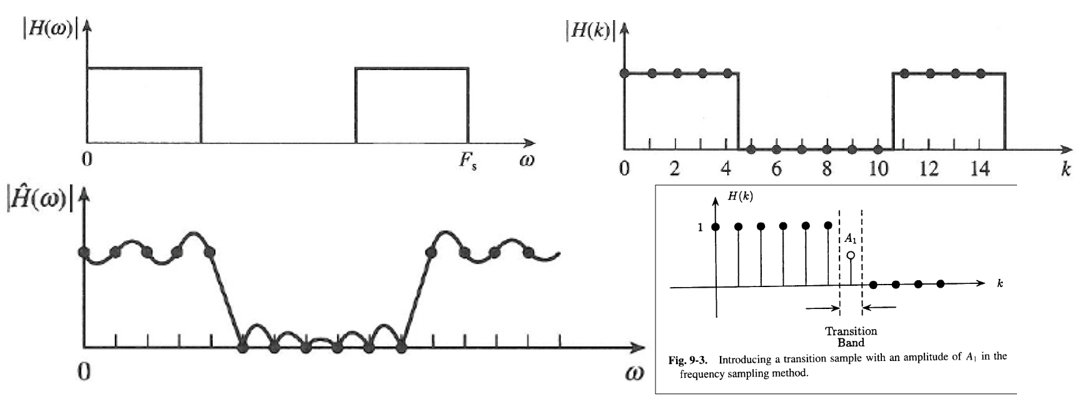
\includegraphics[width=0.75\textwidth]{figures/Filter design/frequency_sampling_method.png}
        \caption{Visual representation of the frequency sampling method}
        \label{fig:freq_sampling_method}
    \end{figure}
    
    \item \textbf{Optimization method:} Use algorithms (e.g. Parks-McClellan) or optimization techniques like least squares to iteratively refine the filter coefficients by minimizing the error between the desired and actual frequency response.
\end{itemize}

\subsubsection{Window functions and the consequences of applying them}
Window functions $w(n)$ are of finite lengths and symmetric around their midpoints. 
\begin{equation}
    \underbrace{h(n)}_{\text{Desired filter}} = \underbrace{h_d (n)}_{\text{Ideal filter}} \ast \ w(n)
\end{equation}
Or in the frequency domain:
\begin{equation}
    H(e^{j\omega}) =  H_d (e^{j\omega}) \circledast W(e^{j\omega}) = \frac{1}{2\pi} \int_{-\pi}^{\pi} H_d (e^{j\nu}) W(e^{j(\omega - \nu)}) d\nu
\end{equation}
\begin{figure}[h!]
    \centering
    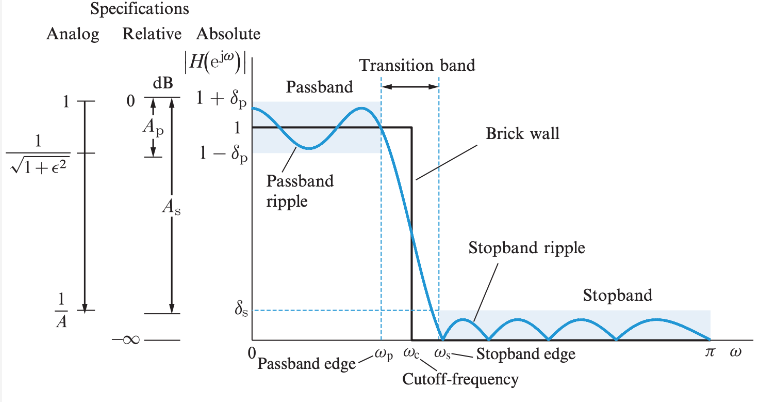
\includegraphics[width=0.75\textwidth]{figures/Filter design/lowpass_tolerance_diagram.png}
    \caption{Example of a lowpass filter tolerance diagram}
    \label{fig:tolerance_diagram}
\end{figure}

How well $H(e^{j\omega})$ approximates $H_d (e^{j\omega})$ is determined by:
\begin{itemize}
    \item The width of the main lobe of $W(e^{j\omega})$
    \item Maximum side lobe level of $W(e^{j\omega})$
\end{itemize}

This method also lacks precise control of $w_p$ and $w_s$.

\paragraph{Some characteristics of window spectrum:}
\begin{itemize}
    \item Pass and stopband ripples are not constant
    \item Stopband level (filter) typically less than peak sidelobe level (PSL) to window. 
    \item PSL, peak passband ripple and passband attenuation $\approx$ independent of $N$.
    \item Width of transition band $\approx$ given by main lobe width window, $F_{WS} \approx C/N$ where $C$ is a constant for each window.
\end{itemize}

\subsubsection{Linear phase and linear-phase filters}
A LTI system has a \textbf{linear phase} if:
\begin{equation}
    H(e^{j\omega}) = |H(e^{j\omega})|e^{-j\alpha\omega}
\end{equation}
Or a \textbf{generalized linear phase} if:
\begin{equation}
    H(e^{j\omega}) = A(e^{j\omega})e^{-j(\alpha\omega - \beta)}
\end{equation}
Where $A(e^{j\omega})$ is a real-valued function of $\omega$ and $\beta \in \mathfrak{R} $
\\
\\
If your system needs to both be \textbf{causal} and have \textbf{linear phase}, you can only use \textbf{FIR}.
\\
\\
A sufficient condition for a real-valued FIR filter to have generalized linear phase is that its impulse response $h(n)$ is symmetric or antisymmetric.
\begin{itemize}
    \item \textbf{Symmetric:} $h(n) = h(M-1-n), \quad n=0,1,\ldots,M-1$
    \\
    Then $\alpha = (M-1)/2$ and $\beta = 0 \ \vee \ \pi$
    \item \textbf{Antisymmetric:} $h(n) = -h(M-1-n), \quad n=0,1,\ldots,M-1$
    \\
    Then $\alpha = (M-1)/2$ and $\beta = \pi/2 \ \vee \ 3\pi/2$
\end{itemize}
For a real linear phase FIR filter with a zero $z_1$, you also have zeros at $z_1^\ast, \frac{1}{z_1}$ and $\frac{1}{z_1^\ast}$
\begin{figure}[h!]
    \centering
    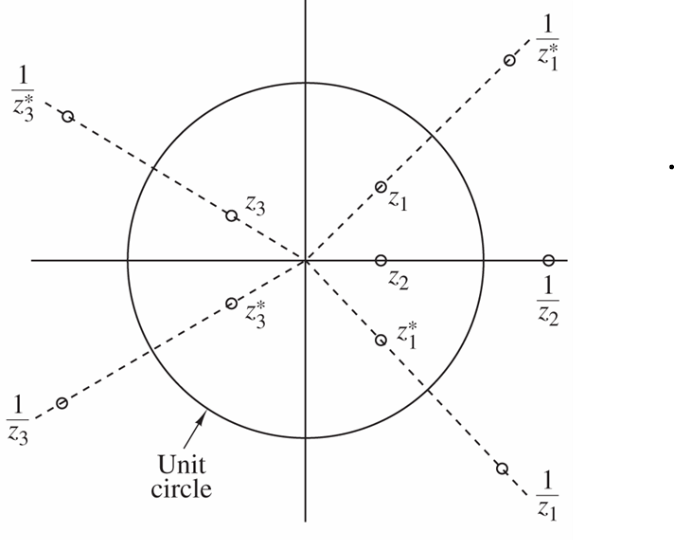
\includegraphics[width=0.4\textwidth]{figures/Filter design/zero_location_FIR.png}
    \caption{Example showing zero symmetry in a FIR filter}
    \label{fig:zero_location_FIR}
\end{figure}

\clearpage

\subsubsection{Graphical representation of filter structures and operations}

\begin{figure}[h!]
    \centering
    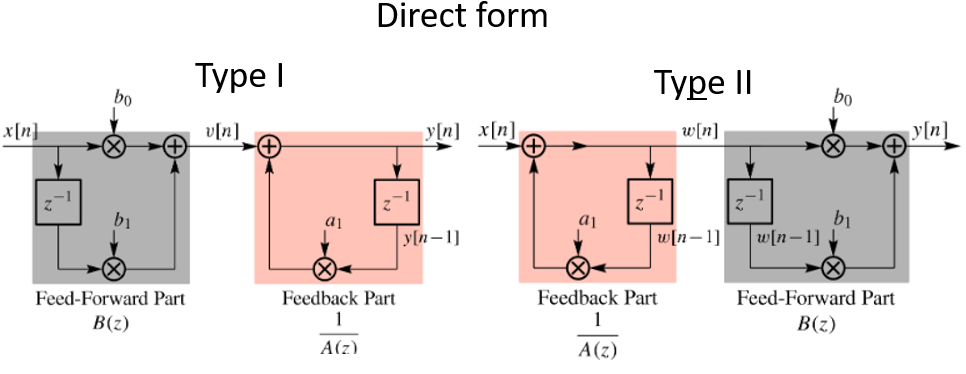
\includegraphics[width=0.75\textwidth]{figures/Filter design/structure_forms.png}
    \caption{Example of a filter structure}
    \label{fig:filter_structure}
\end{figure}

\paragraph{Operator notation:} The $z^{-1}$ blocks in fig.~\ref{fig:filter_structure} are called \textbf{delay operators} and are used to represent the delay of one sample. I.e. $x[n-1] \begin{smallmatrix} \mathcal{Z} \\ \longleftrightarrow \end{smallmatrix} z^{-1}X(z)$

\paragraph{How is it made} Given a transfer function: \[H(z) = \frac{Y(z)}{X(z)} = (b_0 + b_1z^{-1} \ldots) \left( \frac{1}{1-a_1z^{-1} \ldots} \right) = B(z)\frac{1}{A(z)}\]
Note we have two forms, \textbf{direct form I} and \textbf{direct form II}. The later saves one unit delay.

\begin{figure}[h!]
    \centering
    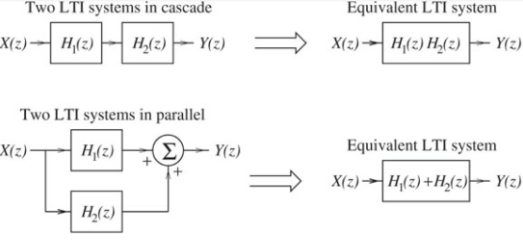
\includegraphics[width=0.6\textwidth]{figures/Filter design/connected_systems.png}
    \caption{Illustration of connected systems}
    \label{fig:connected_systems}
\end{figure}
Figure~\ref{fig:connected_systems} shows how a equivalent transfer function of systems in cascade is the product of the individual transfer functions. The equivalent transfer function of systems in parallel is the sum of the individual transfer functions.

\subsubsection{Gibb's phenomenon}

\begin{itemize}
    \item Oscillatory behavior in the magnitude response of causal FIR filters found by truncating the filter coefficients of an ideal filter.
    \item If you increase the length of the filter, the number of ripple-peaks will increase in both passband and stopband and the width of these peaks decrease equivalent.
    \item Given the same weighting function, the highest ripple-peak will be unchanged. 
\end{itemize}
\begin{figure}[h!]
    \centering
    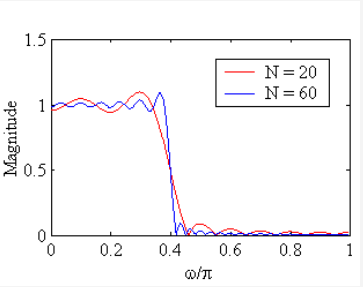
\includegraphics[width=0.75\textwidth]{figures/Filter design/gibbs_effekt.png}
    \caption{Example of Gibb's effect in a lowpass filter}
    \label{fig:gibbs_effect}
\end{figure}

\clearpage

\subsection{Sampling and reconstruction}
\subsubsection{Sampling theorem}
The sampling frequency $\Omega_T = 2\Omega_H$ is called the Nyquist frequency. If this term is satisfied, then the original signal can be recovered from the sampled signal. In practice we often use oversampling (sampling at a higher rate than the Nyquist frequency) to get an appropiate reconstruction.
\subsubsection{Synthesizing an arbitrary signal as a sum of unit impulses}

Sampling corresponds to multiplying with a Dirac comb with distance $T$ between the unit impulses.
In the Fourier domain, this corresponds to convolving with a Dirac comb with distance $F_T$ between
scaled unit impulses. (The distance is $\Omega_T$ if we look at the angular frequency axis)
\begin{figure}[h!]
    \centering
    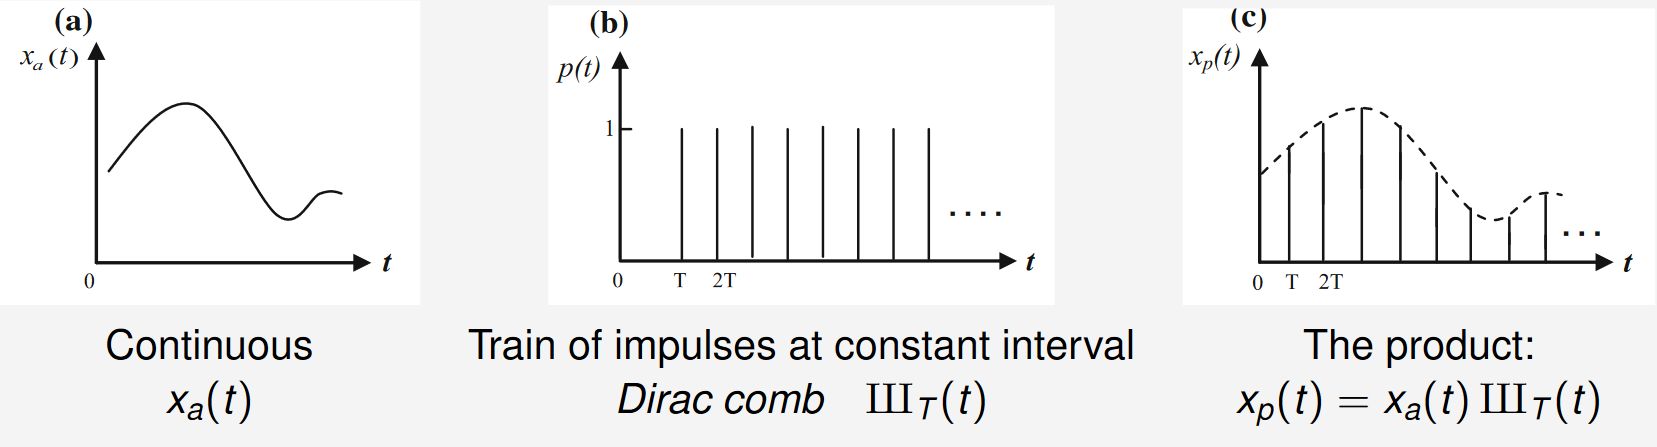
\includegraphics[width=1\textwidth]{figures/Sampling and reconstruction/Sampling_dirac_impulses.png}
    \caption{Sampling with dirac impulses}
    \label{fig:sampling_dirac_impulses}
\end{figure}
\begin{equation}
    x_p (t) = x_a (t) III_T (t) = \sum_{n=-\infty}^{\infty} x_a (t) \delta (t - nT) = \sum_{n=-\infty}^{\infty} x_a (nT) \delta (t - nT) \triangleq x(n)
\end{equation}

\clearpage
\subsubsection{Sampling of band-limited signals}
\begin{figure}[h!]
    \centering
    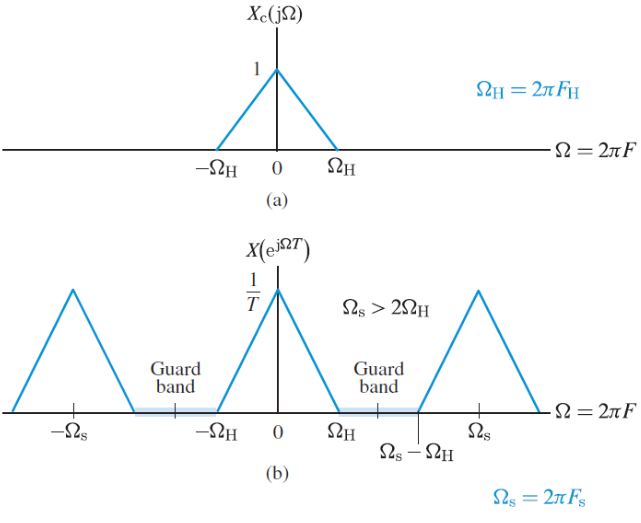
\includegraphics[width=0.75\textwidth]{figures/Sampling and reconstruction/sampling_band_lim_signal.png}
    \caption{Periodic sampling in freq. domain}
    \label{fig:sampling_band_lim_signal}
\end{figure}

\paragraph{Important part:} A signal that is limited to a band $F \in [F_L,F_H]$ is a bandpass with bandwidth $B = F_H - F_L$. This signal can be perfectly reconstructed if $2B \le F_T \le 4B$

\paragraph{Not important}The reconstructed signal will repeat itself in the frequency domain. As long the sampling frequency ($\Omega_T$)is equal or greater than the Nyquist rate ($2\Omega_H$), we will be able to seperate the original signal from the aliases. The reconstruction in fig. \ref{fig:sampling_band_lim_signal} can be written as a convolution:
\begin{equation}
    x_r (t) = \sum_{n=-\infty}^{\infty} x_a (nT) g_r (t - nT) 
\end{equation}

Where $g_r (t)$ is the interpolation reconstruction function (I.e. impulse response). 

\subsubsection{Ideal reconstruction}

The fundamental copy of the Fourier-domain representation of the sampled signal can be found by the 'ideal' filter for the convolution operation is: 
\begin{equation}
    G_r (j\Omega) = \bigg\{ \begin{matrix}
        T, & |\Omega| \leq \Omega_T /2 \\
        0, & |\Omega| > \Omega_T / 2
    \end{matrix}
\end{equation}

This gives the ideal: $X_r (j\Omega) = X_a (j\Omega)$ \\ (Reconstructed Fourier domain representation equals the original Fourier domain representation).

\clearpage
\subsubsection{Upsampling and downsampling}

\begin{figure}[h!]
    \centering
    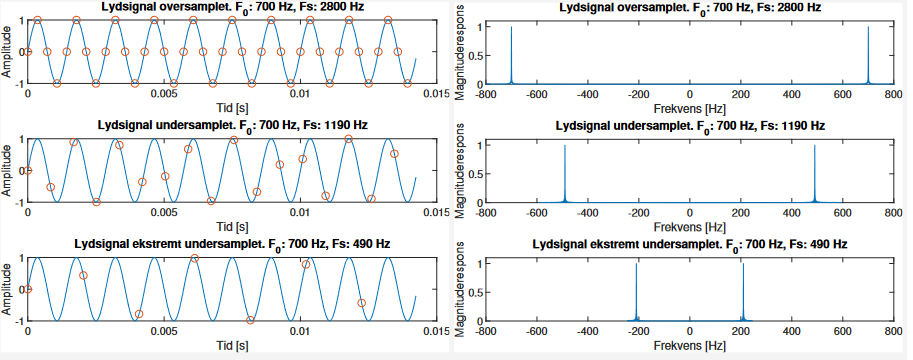
\includegraphics[width=1\textwidth]{figures/Sampling and reconstruction/sampling_examples.png}
    \caption{Example of over/undersampling}
    \label{fig:sampling_example}
\end{figure}

 By upsampling or downsampling we can obtain a new sampled signal with a different sampling frequency.
 We call the new sampled signal $x_0 = x_c(nT_0)$ which is different from the `normal' sampled signal $x(n) = x_c(nT)$.

\paragraph{Downsampling:} $T_0 = DT$ where $D$ is an integer. This is called decimation

\paragraph{Upsampling:} $T_0 = \frac{T}{I}$ where $I$ is an integer. This is called interpolation.
\section{Additional Topics}
\subsection{Discrete time}
\subsubsection{Symmetrical signals}

\paragraph{Symmetrical signal:} A real-valued signal $x(n)$ is said to be symmetric (even) if it satisfies the condition:
\begin{equation}
    x(-n) = x(n)
\end{equation} 
\begin{figure}[h!]
    \centering
    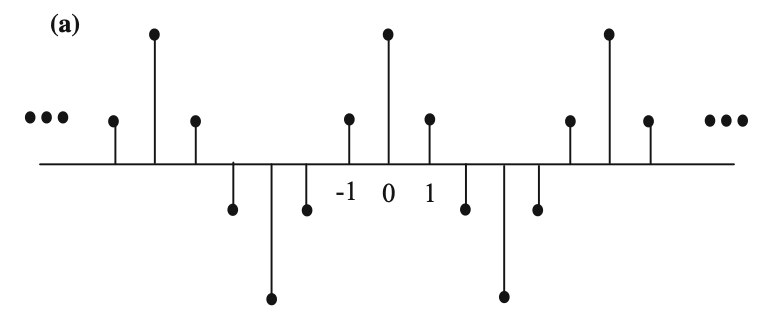
\includegraphics[width=0.75\textwidth]{figures/Discrete time/symmetric_signal.png}
    \caption{Example of a symmetrical signal}
    \label{fig:symmetrical_signal}
\end{figure}

\paragraph{Anti-symmetrical signal:} A real-valued signal $x(n)$ is said to be antisymmetric (odd) if it follows the condition:
\begin{equation}
    x(-n) = -x(n)
\end{equation} 
\begin{figure}[h!]
    \centering
    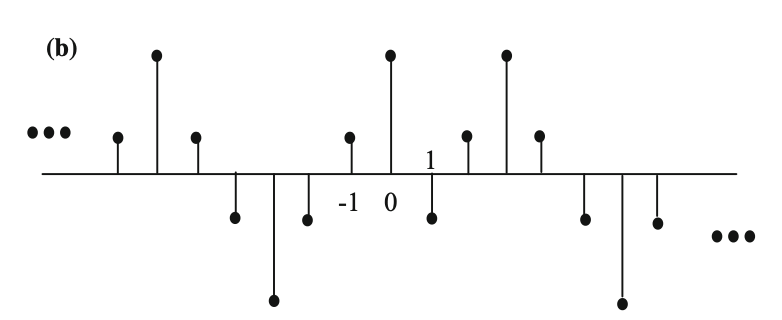
\includegraphics[width=0.75\textwidth]{figures/Discrete time/asymmetric_signal.png}
    \caption{Example of a anit-symmetrical signal}
    \label{fig:antisymmetrical_signal}
\end{figure}

\subsubsection{Signal energy}
The total energy of a signal $x(n)$, real or complex, is defined as: 
\begin{equation}
    E_s = \sum_{n=-\infty}^{\infty} |x(n)|^2
\end{equation}
Energy when talking about signal processing is not, stricly speaking, thesame as  the conventional energy in physics and other sciences. The two concepts are, however, closely related, and it is possible to convert from one to the other:
\begin{equation}
    E = \frac{E_s}{Z} = \frac{1}{Z}\int_{-\infty}^{\infty} |x(t)|^2 dt
\end{equation}
where $Z$ represents the magnitude, in appropriate units of measure, of the load driven by the signal.
\\
For example, if $x(t)$ represents the potential (in volts$[V]$) of an electrical signal propagating across a transmission line, then Z would represent the characteristic impedance (in ohms$[\Omega]$) of the transmission line.
\subsubsection{Signal effect}
???
\subsection{LTI systems and characteristics}

\subsubsection{Static / dynamic systems}
\paragraph{Static system:} A system whose output is due to to present input alone is known as static system. The static system is also called the memoryless system. Can be thought of as a purely resistive electrical circuit.

\paragraph{Dynamic system:} A system whose output depens upon the past or future inputs addition to the present input is called the dynamic system. The dynamic system is also known as memory system. Can be thought of as a reactive electrical circuit (Inductors/Capacitors).

\subsubsection{Recursive / non-recursive}
\paragraph{Recursive:} A system is said to be recursive if the system depends on present and past inputs, as well as previous outputs. I.e. the output of the system is fed back into the system. (IIR Filter)

\paragraph{Non-recursive:} A system is said to be non-recursive if the system current output does not depend on previous output. (FIR Filter)

\subsection{Convolution and correlation}
\subsubsection{Correlation}
Correlation is a measure of similarity between two signals. The general formula for correlation is:
\begin{equation}
    \int_{-\infty}^{\infty}x_1(t)x_2(t-\tau)dt
\end{equation}
There are two types of correlation:
\begin{itemize}
    \item \textbf{Auto correlation}: It is defiend as a correlation of a signal with itself. Auto correlation function is a measure of similarity between a signal and its time delayed version.
    \item \textbf{Cros correlation}: It is the measure of similarity between two different signals.
\end{itemize}

\subsubsection{Strategies for convolution evaluation(direct / graphic / . . . )}

\subsection{Z-transform}

\subsection{Frequency analysis and DFT}

\subsection{Filter design}
\subsubsection{Difference between linear phase and generalized linear phase}
Linear phase systems has a perfectly linear phase response across all frequencies. Generalized linear phase system has a linear phase response, or a approximately linear phase response, in a specified range of frequencies. The latter provides more design flexibility but may give some undesired effects in some ranges of frequencies.

\subsubsection{Type I-IV linear phase filters}

\begin{figure}[h!]
    \centering
    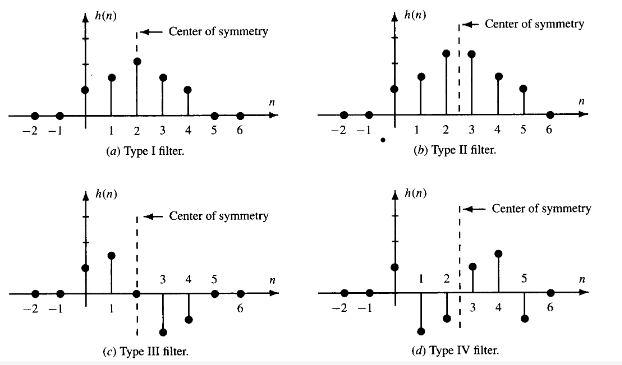
\includegraphics[width=0.75\textwidth]{figures/Filter design/filter_types.png}
    \caption{The different FIR filters}
    \label{fig:filter_types}
\end{figure}

\subsubsection{Mapping between s- and z-plane}
$H(z) = H_a(s) \Big|_{s=m(z)}$

Where $s=m(z)$ is the mapping function with the following properties:
\begin{itemize}
    \item $j\Omega$-axis should be mapped to the unit circle.
    \item Points in the left-half s-plane should be mapped inside the unit circle.
    \item $m(z)$ should be rational so a rational $H_a(s)$ can be mapped to a rational $H(z)$.
\end{itemize} 

\subsubsection{Bi-linear transformation when designing IIR filters}
Mapping from s-plane to z-plane is defined as $s = \frac{2}{T_s}\frac{1-z^{-1}}{1+z^{-1}} \rightarrow H(z)= H_a \left( \frac{1-z^{-1}}{1 + z^{-1}} \right)$.

This mapping is rational, one-to-one and onto, but the nonlinear relations between the $j\Omega$-axis and the unit circle causes warping.

\subsubsection{Result of warping}
Bi-linear mapping will only preserve the magnitude response of analog filter that have an idea response that is piecewise constant.

\subsection{Sampling and reconstruction}
\subsubsection{Up/downsampling with factor that is not an integrer:}
This is done by resampling with the non-integrer factor $I/D$. I.e we upsample with $I$ and then downsample with $D$. 


\paragraph{Notes from group session:}
\begin{itemize}
    \item x(n) is input, y(n) is ouput and h(n) is impulse response. 
    \item FIR filter has to have symmetrical coefficients to have linear phase.
    \item The placement of the zero can give us the magnitude plot. And from the magnitude plot we can see the frequency spectrum. 
    \item Three ways to see if it is causal, ROC or difference equation
    \item From ROC, it is causal if it contains infinity
    \item For n<0, if h(n) (Impulse response) have a postive value, it it anti-causal.
    \item For the DTFT to exists, the unit cicle must lie inside the ROC
\end{itemize}
\end{document}